\documentclass[14pt]{extarticle}

\usepackage[T2A]{fontenc}
\usepackage[utf8]{inputenc}
\usepackage[english,ukrainian]{babel}
\usepackage{bookmark}

\usepackage{amsmath,amssymb}
\usepackage{parskip}
\usepackage{graphicx}
\usepackage[table]{xcolor}
\usepackage{tcolorbox}
\tcbuselibrary{skins}
\usepackage[framemethod=tikz]{mdframed}
\usepackage{chngcntr}
\usepackage{enumitem}
\usepackage{hyperref}
\usepackage{float}
\usepackage{subfig}
\usepackage{chngcntr}
\usepackage{esint}
\usepackage{pdfpages} % Add this to your preamble

\usepackage{libertinus}

\usepackage[top=2.5cm, left=3cm, right=3cm, bottom=4.0cm]{geometry}
\usepackage{algorithm}
\usepackage{algpseudocode}
\usepackage{listings}
\usepackage{xcolor}

\definecolor{codegreen}{rgb}{0,0.6,0}
\definecolor{codegray}{rgb}{0.5,0.5,0.5}
\definecolor{codepurple}{rgb}{0.58,0,0.82}
\definecolor{backcolour}{rgb}{0.95,0.95,0.92}

\lstdefinestyle{mystyle}{
    backgroundcolor=\color{backcolour},   
    commentstyle=\color{codegreen},
    keywordstyle=\color{magenta},
    numberstyle=\tiny\color{codegray},
    stringstyle=\color{codepurple},
    basicstyle=\ttfamily\footnotesize,
    breakatwhitespace=false,         
    breaklines=true,                 
    captionpos=b,                    
    keepspaces=true,                 
    numbers=left,                    
    numbersep=5pt,                  
    showspaces=false,                
    showstringspaces=false,
    showtabs=false,                  
    tabsize=2
}
\lstset{style=mystyle}

\usepackage{ragged2e}
\begin{document}

\begin{titlepage}
	\centering
	%
\includegraphics[width=0.15\textwidth]{images/lab_1/logo.png}\par\vspace{0.3cm}
	{\textbf{Міністерство освіти і науки України}\par
 Харківський національний університет імені В.Н. Каразіна\par}
    \vspace{1cm}
	{\Large \textsc{Розрахунково-графічне завдання \#1}\par
    \textbf{Інтегрування диференціальних рівнянь}\par}
	\vfill
 \begin{FlushRight}
	\textbf{Виконав:}\par Захаров Дмитро Олегович \par Група МП-41
\end{FlushRight}
	\vfill

% Bottom of the page
	{\large Харків -- 2025\par}
\end{titlepage}

\tableofcontents
\pagebreak

\section{Постановка задачі}

Знайти розв'язок задачі Коші
\begin{equation*}
    \begin{cases}
        y' = f(x,y), \; x \in [x_0,b], \\
        y(x_0) = y_0
    \end{cases}
\end{equation*}

в точках $x_i = x_0 + ih$ для $i \in [n]$, $h=(b-x_0)/n$ з точністю $\varepsilon
= 10^{-6}$ за допомогою:
\begin{itemize}
    \item Методу Ейлера;
    \item Методу Рунге-Кутти, використовуючи двійний перерахунок і оцінку за
    Рунге.
\end{itemize}

На друк вивести результати у вигляді таблиці
\begin{itemize}
    \item $x_i$, $y_i := y(x_i)$;
    \item $u_i$ --- найближче значення розв'язку у точці $x_i$.
    \item $|y_i - u_i|$.
\end{itemize}

\textbf{Варіант 5.}
\[
f(x,y) = -2y^2 \ln x - \frac{y}{x}, \quad y(x) = \frac{1}{x(1+\ln^2 x)}.
\]

Параметри $x_0=1$, $b=2$, $y_0=5$, $n=10$.

\pagebreak
\section{Опис методів}

\subsection{Метод Ейлера}

Ітеративно застосовуємо формулу:
\begin{equation*}
    x_{i+1} \gets x_i + h, \quad y_{i+1} \gets y_i + h f(x_i,y_i).
\end{equation*}

Помилка в цьому випадку $\mathcal{O}(h^2)$. Покращений метод Ейлера:
\begin{equation*}
    x_{i+1} \gets x_i + h, \quad y_{i+1} \gets y_i + \frac{h}{2}(f(x_i,y_i) + f(x_{i+1},y_{i+1})).
\end{equation*}

Цей метод дає помилку $\mathcal{O}(h^3)$.

\subsection{Метод Рунге-Кутти}

Ітеративно застосовуємо наступні дії:
\begin{align*}
    (1) &&& y_{i+1} \gets y_i + \frac{1}{6}\left(k_1+2k_2+2k_3+k_4\right), \\
    (2) &&& k_1 \gets hf(x_i,y_i), \\
    (3) &&& k_2 \gets hf(x_i+\frac{1}{2}h,y_i+\frac{1}{2}k_1), \\
    (4) &&& k_3 \gets hf(x_i+\frac{1}{2}h,y_i+\frac{1}{2}k_2), \\
    (5) &&& k_4 \gets hf(x_i+h,y_i+k_3)
\end{align*}

Щоб скористатися оцінкою за Рунге, потрібно паралельно до виконання основного методу
з кроком $h$, виконати його з кроком $h/2$. В такому разі, якщо задати точність 
$\varepsilon$, то ми виконуємо перерахунок до тих пір, поки
\begin{equation*}
    \left|y_j^{(h)} - y_j^{(h/2)}\right| < (2^{\rho}-1)\varepsilon,
\end{equation*}

де $\rho$ -- порядок методу. В нашому випадку $\rho=4$, тому
\begin{equation*}
    \left|y_j^{(h)} - y_j^{(h/2)}\right| < 15\varepsilon.
\end{equation*}

\section{Код програми}
\label{sec:attached-pdf}

Код програми наведений на мові \textit{Wolfram Mathematica} у файлі, 
що прикріплений далі.

\begin{center}
    \textbf{Перегорніть на наступну сторінку $\to$}
\end{center}

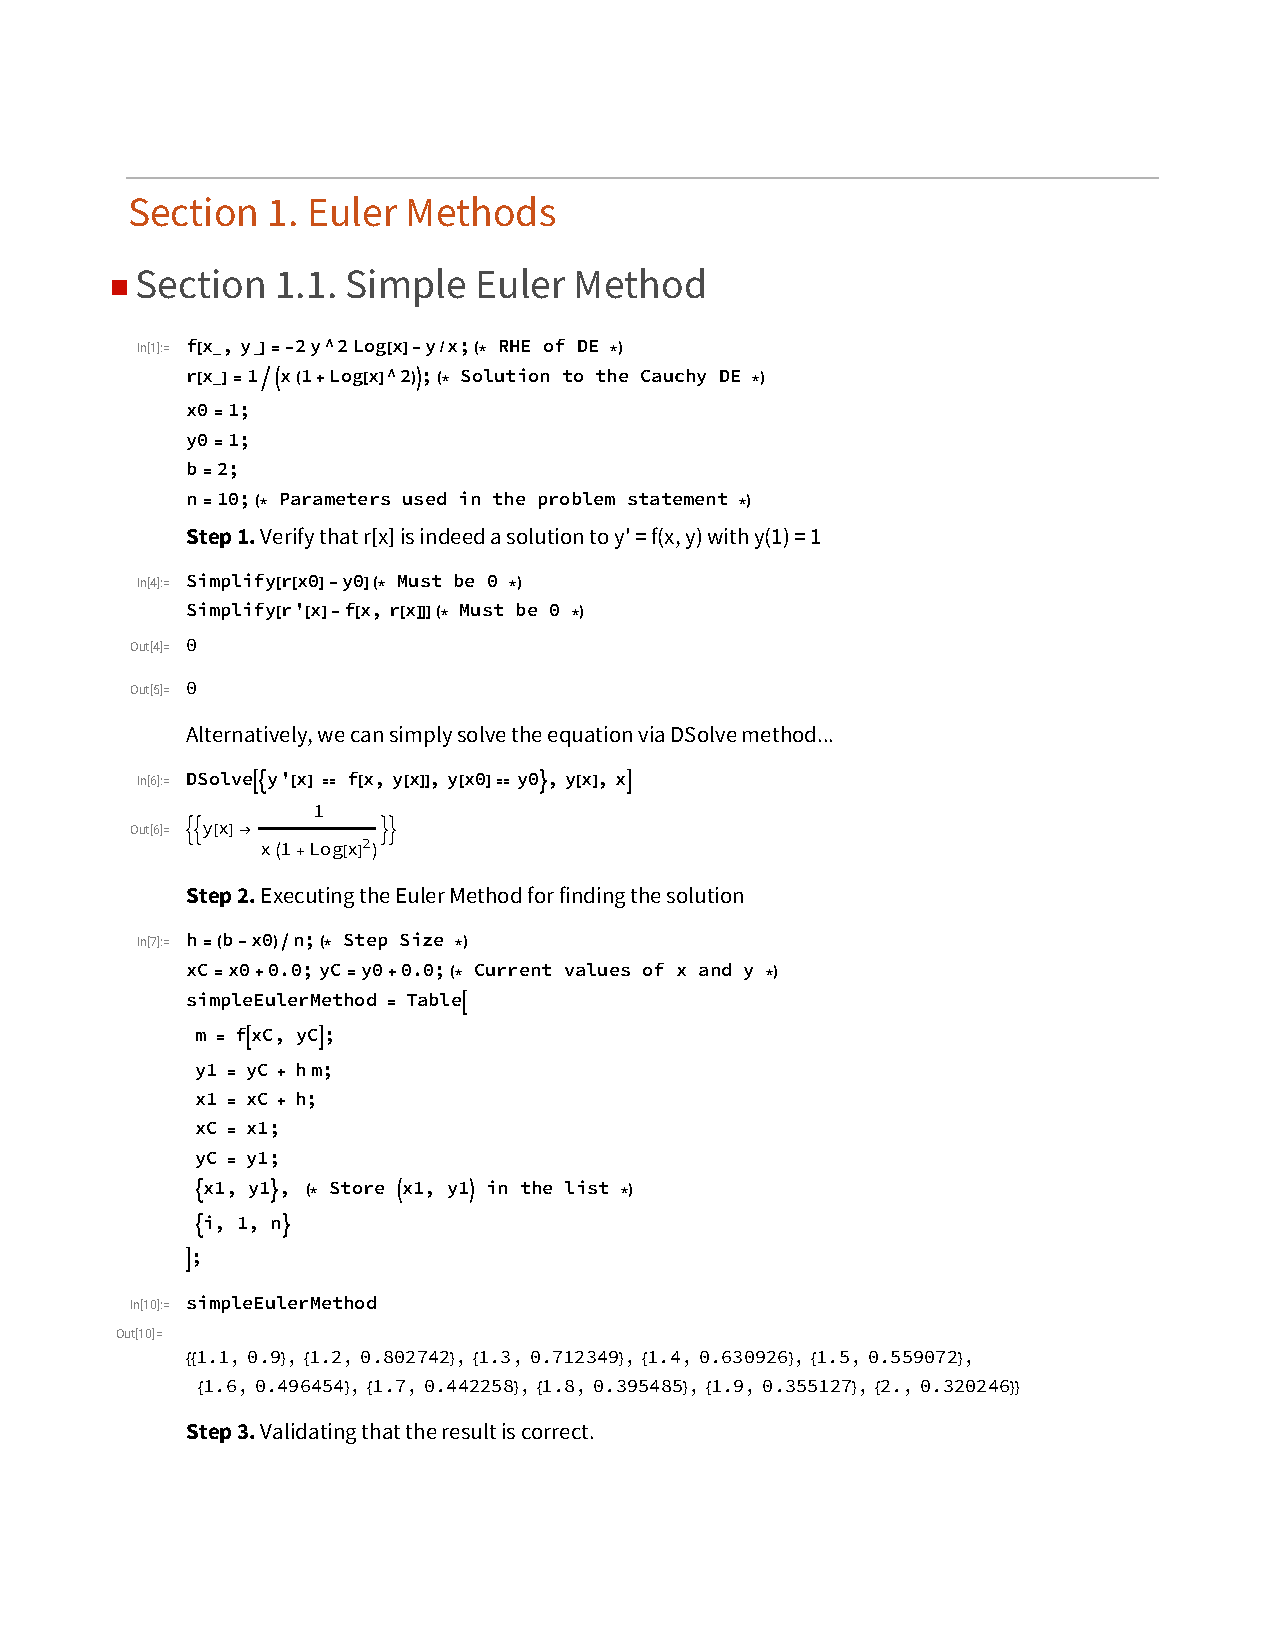
\includepdf[pages=-]{appendices/lecture-1-appendix.pdf}  % `pages=-` includes all pages

\end{document}

